\documentclass[9pt,twocolumn,twoside]{optica}
\setboolean{shortarticle}{false}
\setboolean{minireview}{false}

\title{Legacy \LaTeX\ template for preparing an article for submission to \emph{Optica}}

\author[1,2,*]{Francesca Venturini}
\author[2]{Umberto Michelucci}
\author[1]{Michael Baumgartner}

\affil[1]{Institute of Applied Mathematics and Physics, Zurich University of Applied Sciences,
Technikumstrasse 9, 8401 Winterthur, Switzerland}
\affil[2]{TOELT LLC; Birchlenstr. 25, 8600 Dübendorf, Switzerland}

\affil[*]{Corresponding author: francesca.venturini@zhaw.ch}

% To be edited by editor
% \dates{Compiled \today}

%\ociscodes{(140.3490) Lasers, distributed feedback; (060.2420) Fibers, polarization-maintaining; (060.3735) Fiber Bragg gratings.}

% To be edited by editor
% \doi{\url{http://dx.doi.org/10.1364/optica.XX.XXXXXX}}

\begin{abstract}
This legacy \LaTeX\ template can be used to prepare a research article or a short article for submission to \emph{Optica}. Select \texttt{$\setminus$setboolean\{shortarticle\}\{false\}} for a research article or \texttt{$\setminus$setboolean\{shortarticle\}\{true\}} for a letter or memorandum. Select \texttt{$\setminus$setboolean\{minireview\}\{true\}} to output a header identifying the paper as a Mini-Review. Authors may use this legacy template for a precise length estimate for \emph{Optica} letters and memoranda. Please note that OSA is no longer using OCIS codes.
\end{abstract}

\setboolean{displaycopyright}{true}

\begin{document}

\maketitle

\section{Introduction}

This legacy template is designed to assist with creating a two-column research article or letter to submit to \emph{Optica}. See the OSA's \href{http://www.opticsinfobase.org/submit/style/}{Style Guide} and \href{http://www.opticsinfobase.org/submit/templates/}{Manuscript Templates} pages for more details.

If you have a question while using this template on \href{https://www.overleaf.com}{Overleaf}, please use the help menu (``?'') on the top bar to search for help or ask us a question using the option in the lower right of the editor.

\section{Methods}
\label{sec:methods}


\subsection{Experimental Setup}
\label{Experimental}

To determine the parameters for the synthetic data for the training of the neural network and for the validation of the method several luminescence measurements were performed under varying conditions.

The sample used for the characterization and test is a commercially available Pt-TFPP-based oxygen sensor spot (PSt3, PreSens Precision Sensing GmbH, Regensburg, Germany).
To control the temperature of the samples, these were placed in good thermal contact with a copper plate, placed in a thermally insulated chamber. The temperature of this plate was adjusted at a fixed value between 0 $^\circ$C and 45 $^\circ$C using a Peltier element and stabilized with a temperature controller (PTC10, Stanford Research Systems, Sunnyvale, CA USA). The thermally insulated chamber was connected to a self-made gas-mixing apparatus which enabled to vary the oxygen concentration between 0 $\%$ and 20 $\%$ vol $O_2$ by mixing nitrogen and dry air. In the following, the concentration of oxygen will be given in $\%$ of the oxygen concentration of dry air and indicated with $\%$ air. This means, for example, that 20 $\%$ air corresponds to 4 $\%$ vol $O_2$ and 100 $\%$ air corresponds to 20 $\%$ vol $O_2$.  
The absolute error on the oxygen concentration adjusted with the gas mixing device is estimated to be below 1 $\%$ air. 

The optical setup used in this work for the luminescence measurements is shown schematically in Fig. \ref{fig:setup}.
\begin{figure}[t]
\centering
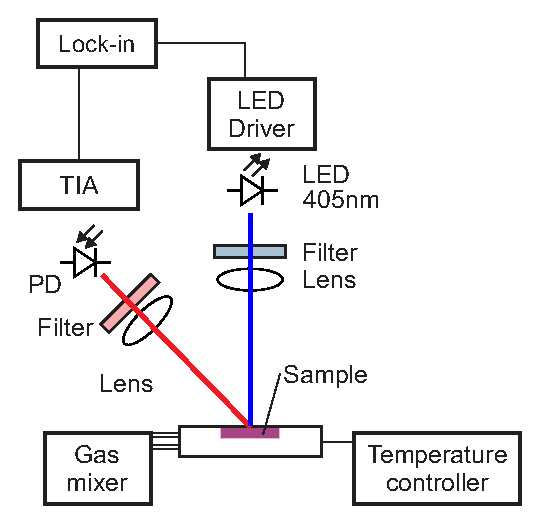
\includegraphics[keepaspectratio, width=7.5cm]{Figures/setup}
\caption{Scheme of the optical experimental setup. Blue is the excitation, red the luminescence optical path. PD: photodiode; TIA: trans-impedance amplifier.}
\label{fig:setup}
\end{figure}
The excitation light was provided by a 405 nm LED (VAOL-5EUV0T4, VCC Visual Communications Company, LLC, San Marcos, CA USA), filtered by a an OD5 short pass filter with cut-off at 498 nm (Semrock 498 SP Bright Line HC short pass, Semrock, Inc., Rochester, NY, USA) and focused on the surface of the samples with a collimation lens (EO43987, Edmund Optics, Tucson, AZ USA). The luminescence was focussed by a lens (G063020000, LINOS, Qioptiq, Göttingen, Germany) and collected by a photodiode (SFH 213 Osram, Opto Semiconductors GmbH,  Regensburg, Germany).
To suppress stray light and light reflected by the sample surface, the emission channel was equipped with an OD5 long pass filter with cut-off at 594 nm (Semrock 594 LP Edge Basic long pass, Semrock, Inc., Rochester, NY, USA) and an OD5 short pass filter with cut-off at 682 nm (Semrock 682 SP Bright Line HC short pass, Semrock, Inc., Rochester, NY, USA). The driver for the LED and the trans-impedance amplifier (TIA) are self-made.
For the frequency generation and the phase detection a two-phase lock-in amplifier (SR830, Stanford Research Inc.) was used. The modulation frequency was varied between 200 Hz and 20 kHz.



The sections below show examples of different article components. Sections should generally follow the conventional order: Introduction, Method, Results, Discussion, and Conclusion.  Please do not include Methods in a separate section at the end.

\begin{figure}[hbt]
\centering
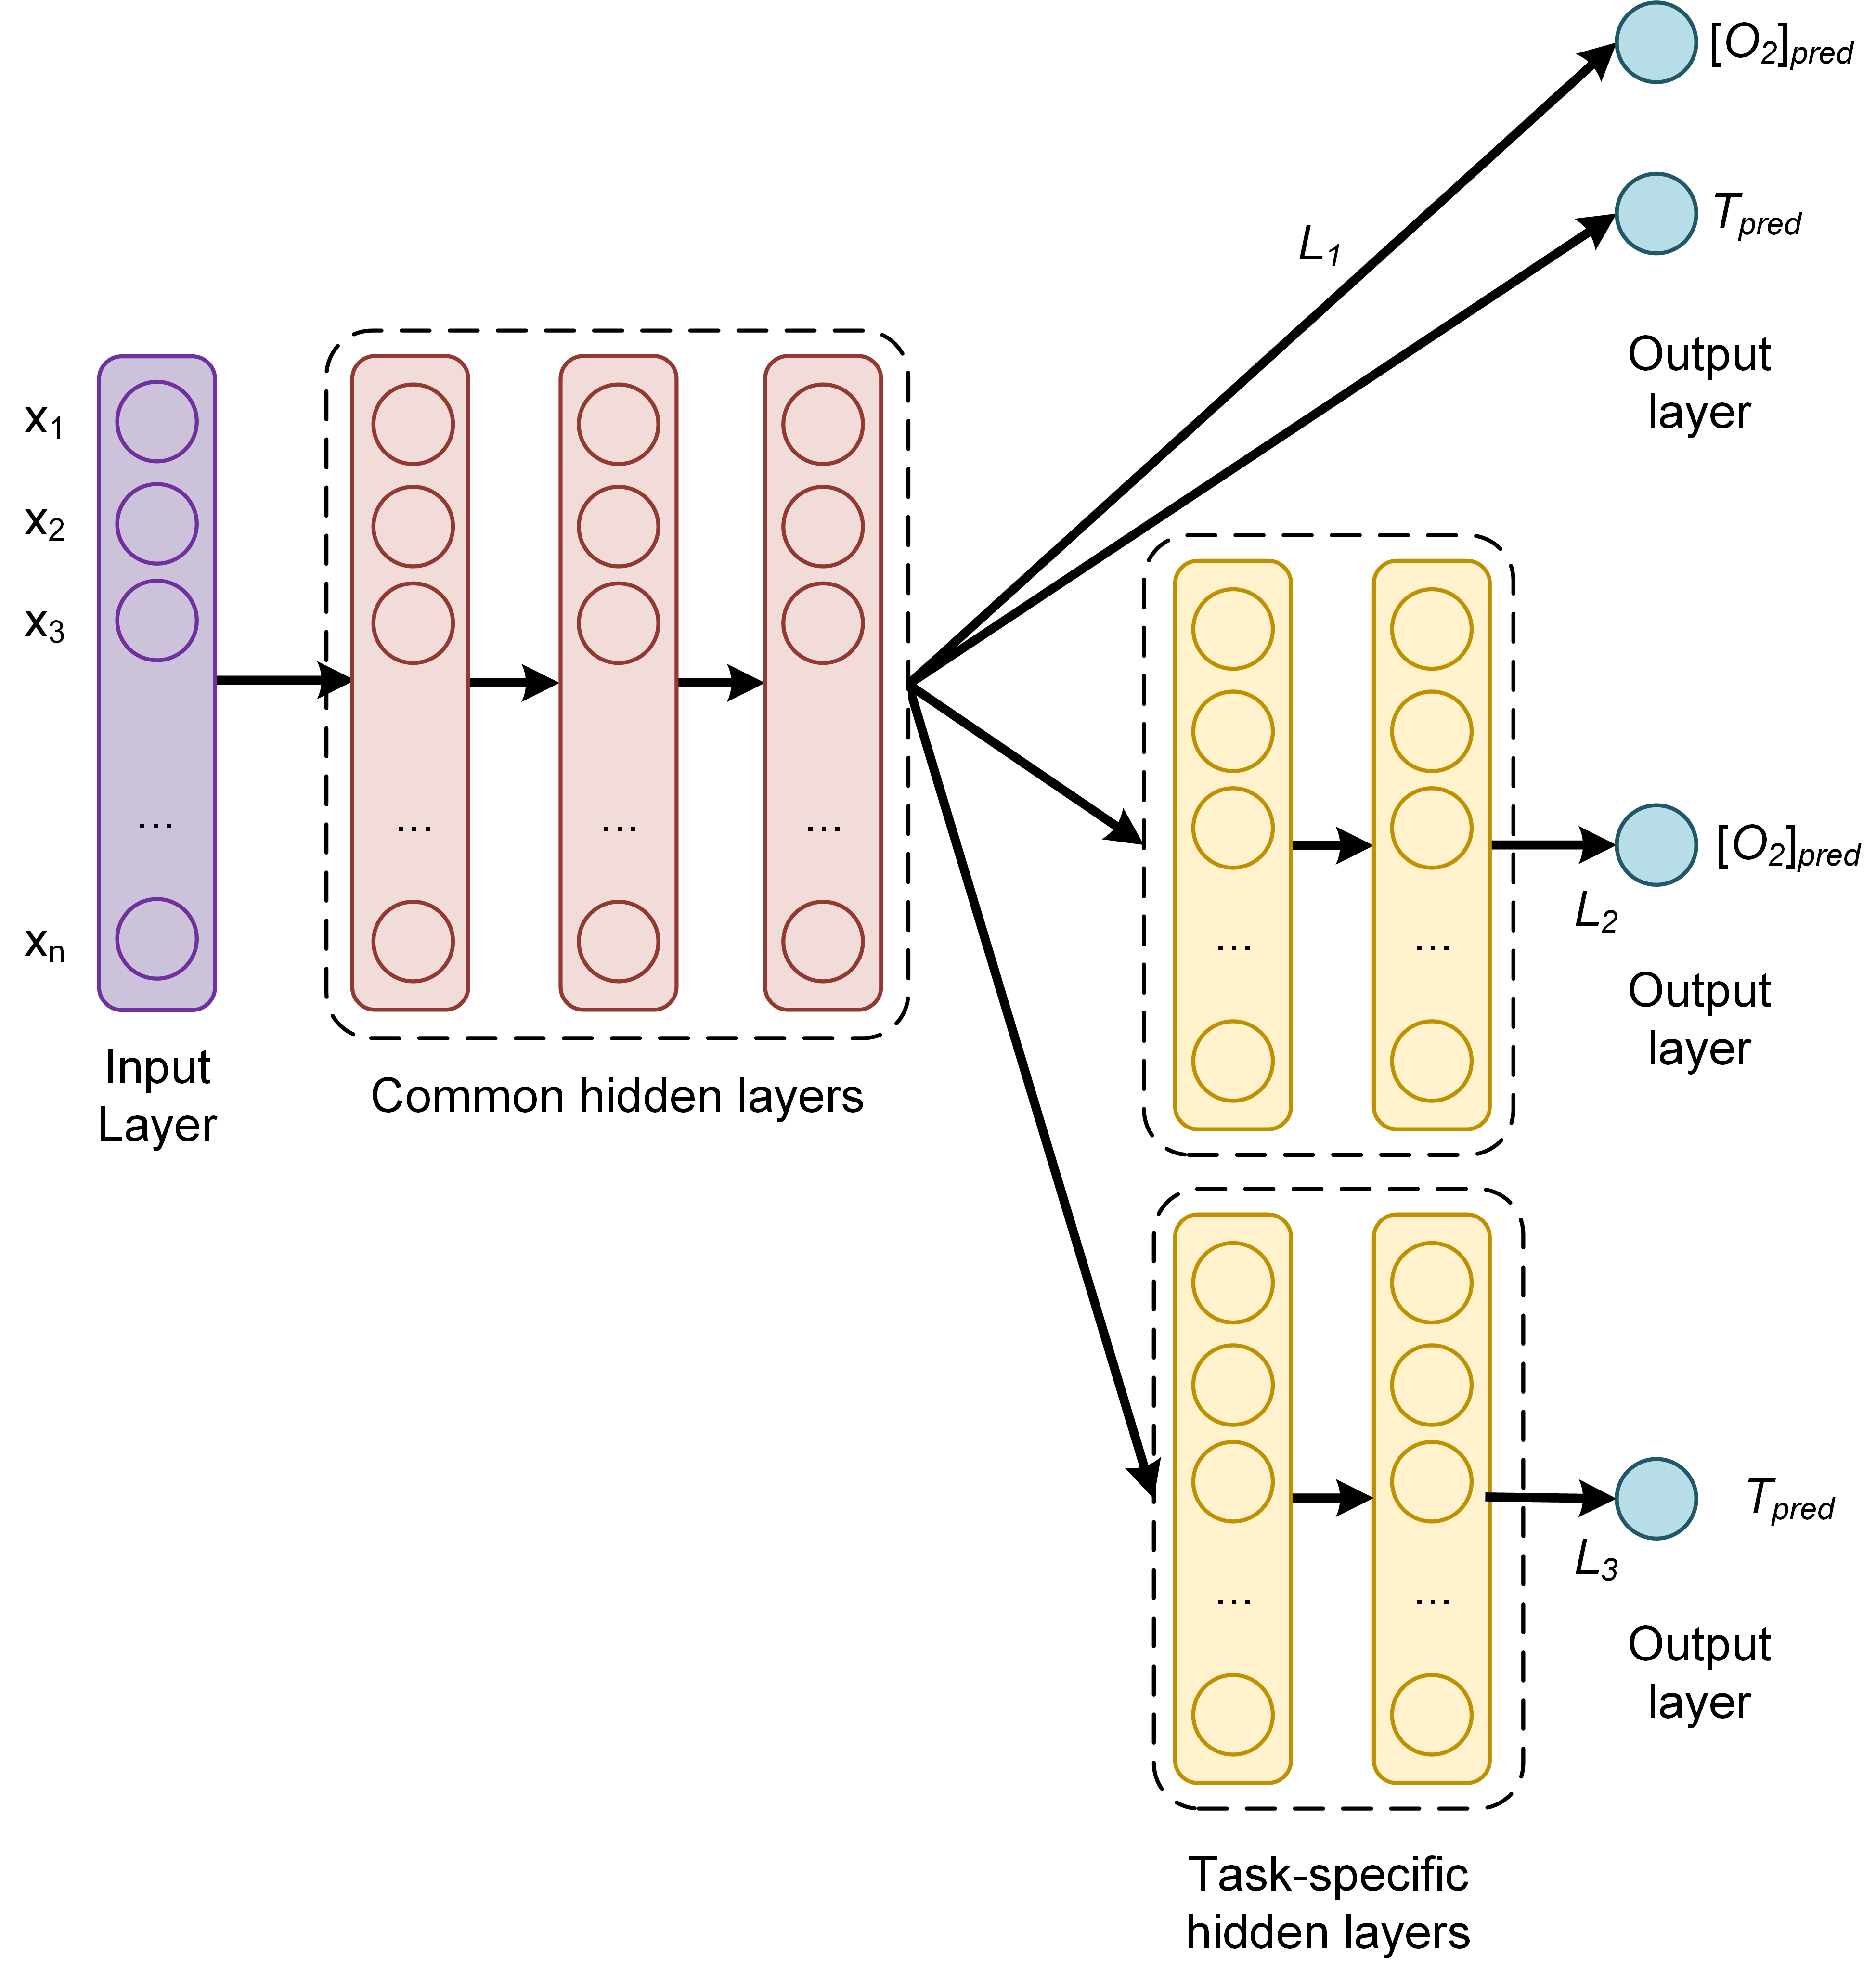
\includegraphics[width=9 cm]{figures/NN_MTL_O2_T.png}
\caption{Architecture of the feed-forward MTL network C.}
\label{NN_MTL_O2_T}
\end{figure}


\section{Results}



\subsection{Figures and Tables}

Figure \ref{fig:false-color} shows an example figure.

\begin{figure}[htbp]
\centering
\fbox{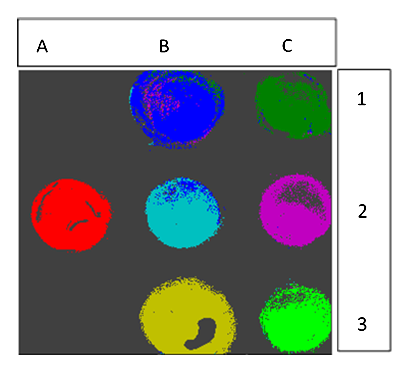
\includegraphics[width=\linewidth]{sample}}
\caption{False-color image, where each pixel is assigned to one of seven reference spectra.}
\label{fig:false-color}
\end{figure}

\subsection{Sample Table}

Table \ref{tab:shape-functions} shows an example table.

\begin{table}[htbp]
\centering
\caption{\bf Shape Functions for Quadratic Line Elements}
\begin{tabular}{ccc}
\hline
local node & $\{N\}_m$ & $\{\Phi_i\}_m$ $(i=x,y,z)$ \\
\hline
$m = 1$ & $L_1(2L_1-1)$ & $\Phi_{i1}$ \\
$m = 2$ & $L_2(2L_2-1)$ & $\Phi_{i2}$ \\
$m = 3$ & $L_3=4L_1L_2$ & $\Phi_{i3}$ \\
\hline
\end{tabular}
  \label{tab:shape-functions}
\end{table}

\section{Results}

Let $X_1, X_2, \ldots, X_n$ be a sequence of independent and identically distributed random variables with $\text{E}[X_i] = \mu$ and $\text{Var}[X_i] = \sigma^2 < \infty$, and let
\begin{equation}
S_n = \frac{X_1 + X_2 + \cdots + X_n}{n}
      = \frac{1}{n}\sum_{i}^{n} X_i
\label{eq:refname1}
\end{equation}
denote their mean. Then as $n$ approaches infinity, the random variables $\sqrt{n}(S_n - \mu)$ converge in distribution to a normal $\mathcal{N}(0, \sigma^2)$.

\section{Conclusions}



%\section*{Funding Information}
%National Science Foundation (NSF) (1263236, 0968895, 1102301); The 863 Program (2013AA014402).

%\section*{Acknowledgments}


\section*{Disclosures}

\medskip

\noindent\textbf{Disclosures.} The authors declare no conflicts of interest.

\section*{Supplemental Documents}
\emph{Optica} authors may include supplemental documents with the primary manuscript. For details, see \href{http://www.opticsinfobase.org/submit/style/supplementary-materials-optica.cfm}{Supplementary Materials in Optica}. To reference the supplementary document, the statement ``See Supplement 1 for supporting content.'' should appear at the bottom of the manuscript (above the references).

%\bigskip \noindent See \href{link}{Supplement 1} for supporting content.

\section*{References}

For references, you may add citations manually or use BibTeX. E.g. \cite{Zhang:14}.

Letter submissions to \emph{Optica} require two sets of references: an abbreviated reference style for publication and a full reference list to aid the editor and reviewers. Citations to journal articles in the abbreviated list should omit the article title and final page number; this abbreviated reference style is produced automatically when the \texttt{$\setminus$setboolean\{shortarticle\}\{true\}} option is selected in the template, if you are using a .bib file for your references.
 
The full reference list meant to aid the editor and reviewers must be included as well on an informational page that will not count against page length; again this will be produced automatically if you are using a .bib file and have the \texttt{$\setminus$setboolean\{shortarticle\}\{true\}} option selected.


% Bibliography
\bibliography{sample}

% Full bibliography will be added automatically on a new page for Optics Letters submissions. This command is ignored for journal article submissions.
% Note that this extra page will not count against page length.
\bibliographyfullrefs{sample}

%Manual citation list
%\begin{thebibliography}{1}
%\bibitem{Zhang:14}
%Y.~Zhang, S.~Qiao, L.~Sun, Q.~W. Shi, W.~Huang, %L.~Li, and Z.~Yang,
 % \enquote{Photoinduced active terahertz metamaterials with nanostructured
  %vanadium dioxide film deposited by sol-gel method,} Opt. Express \textbf{22},
  %11070--11078 (2014).
%\end{thebibliography}

\end{document} 